\documentclass[a4paper,twoside]{article}
\usepackage[hmarginratio=1:1,top=32mm,columnsep=20pt]{geometry} % custom page layout
\usepackage[T1]{fontenc}
\usepackage[utf8]{inputenc}
\usepackage[english]{babel}
\usepackage{lmodern}
\usepackage{fixltx2e} % \textsubscript command
\usepackage{soulutf8} % \ul command
\usepackage{changepage} % indentation (in title page)
\usepackage[font=it]{caption} % captions in italics
\usepackage[font=it]{subcaption} % subcaptions in italics
\usepackage{multicol}
\usepackage{cancel} % \cancel command
\usepackage{textcomp} % symbols
\usepackage{amsmath, amssymb}
\usepackage{amsthm}
\usepackage{makeidx}
\usepackage{graphicx}
\usepackage{float}
\usepackage{listings}
\usepackage{mips}


\usepackage{verbatim}
\lstset{language=[mips]Assembler,%
	  keywordstyle=\color{Blue},
      basicstyle=\small\ttfamily,
      frame=TB,
      %commentstyle=\color{red},
      showstringspaces=false,
      commentstyle=\color{Gray}
}
\usepackage[dvipsnames,usenames]{color}
\usepackage{fancyhdr}



\pagestyle{fancy}
%\renewcommand{\chaptermark}[1]{\markboth{#1}{}}
\renewcommand{\sectionmark}[1]{\markright{\thesection \space - \space #1}}
\renewcommand{\subsectionmark}[1]{\markright{\thesubsection \space - \space #1}}
\fancyhf{} \fancyhead[RO, LE]{\bfseries\thepage}
\fancyhead[CO, CE]{\bfseries\rightmark}
%\fancyhead[CE]{\bfseries \leftmark}
\renewcommand{\headrulewidth}{0.5pt}
\renewcommand{\footrulewidth}{0pt}
\addtolength{\headheight}{0.5pt} \fancypagestyle{plain}{
\fancyhead{}
\renewcommand{\headrulewidth}{0pt}}

\newtheorem{thm}{Teorema}[section] 
\newtheorem{cor}[thm]{Corollario} 
\newtheorem{lem}[thm]{Lemma} 
\newtheorem{prop}[thm]{Proposizione} 
\theoremstyle{definition} 
\newtheorem{defn}{Definizione}[section]
\theoremstyle{remark} 
\newtheorem{oss}{Osservazione} 
\frenchspacing
\author{Alessandro Salvato}

\newcommand{\paginavuota}{\newpage\null\thispagestyle{empty}\newpage\null}

\begin{document}

\thispagestyle{empty}
\begin{center}
\text{\LARGE{\textbf{Paolo Monti}}}\space\space\space\space\space\text{\LARGE{\textbf{Alessandro Salvato}}}\space\space\space \text{\LARGE{\textbf{  Michele Simili}}}
\end{center}
$\\$
\begin{figure}[H]
\centering

\includegraphics[scale=.3]{Immagini/262}
\label{262}
\end{figure}
\begin{center}
\LARGE { \textbf {POLITECNICO DI TORINO} }\\ [1\baselineskip]
%Raccolta di Appunti \\ [2\baselineskip]
\huge{ \textbf{Computer Architectures}}\\ [1\baselineskip]
\Huge{\textbf{Defeating Hardware Trojan through Software Obfuscation}}\\[1\baselineskip]


\end{center}

\begin{flushleft}
\large{Professor: Ernesto Sanchez}
\end{flushleft}
\begin{flushleft}
\large{Data: \today}
\end{flushleft}

\clearpage
\paginavuota

\tableofcontents
\newpage

\section{Introduction}

Due to the increasing costs of manufacturing chips smaller and smaller transistors, the vast majority of companies is forced to employ and trust a third party to fabricate their design. This makes them very susceptible to malicious circuitry injected into their chip at fabrication time. We want to focus on digital hardware that can cause unintended behaviour (trojan). The project is divided into two parts: understanding how a digital hardware trojan works by developing an example, and how to mitigate or deny its malicious effects. This report will focus on the second part only.
This final report aims at gathering the result of applying an evolutionary algorithm, run by uGP3, to some assembly programs (study cases) in a miniMips environment, in order to avoid the activation of an hardware trojan inside it. Our prototype trojan raises a payload when a certain sequence of instructions I1-I2-I3 is detected. Obviously, we don't know the exact sequence, so our aim is to mitigate the activation of a trojan triggered by an unknown sequence. \newline
The starting population generated by uGP is a sequence of integers, between 0 and 99, one for each line of the starting code. Each one of there numbers represent a gene of the individual, effectively making up its DNA. \newline
Then, the external evaluator takes control, with the final aim of defining the fitness values for the given individual. These parameters are 3, and uGP aims at maximizing them all in a multi-objective way.\newline
First of all, the starting code is modified according to the DNA of the individual, with some rules defined in the codeShuffler.py script. The basic operations that can be applied to a line of code are 3. The first one simply adds a line with a NOP instruction, that where the processors does nothing relevant. The second one swaps the current line with the line above or below it. The last one, which is the most important, substitutes a line of code with one or more lines that are equivalent, i.e. they have the same output. The rules for substitution of an instruction can be found in Appendix A. \newline
Applying all these rules, a new source file, modifiedCode.src, is generated. This file is now taken by the miniMips assembler and converted into a binary file. \newline
The code is then simulated by the miniMips processor and some data is collected. Specifically, we are interested about the state of the data memory at the end of the simulation, the total elapsed time, and the number of accesses made to the memory by load and store instructions.\newline
This information is then taken by another script, that finally computes the fitness based on their values. The most important thing is checking that the output of the program is the same as the one of the starting program. If they are different, the individual is discarded by setting its fitness values to 0. If their outputs are the same, the Jaccard Index between startingCode and modifiedCode is computed. The Jaccard Index is a parameter that represents how much different two text files are. In our case, it is very useful because it allows to check whether or not the new code has really changed. \newline
Once it is computed, the final fitness indicators are the Jaccard Index, the reciprocal of the simulation time, and the reciprocal of the number of memory accesses. The last two are reciprocated because the evolutionary algorithm aims at maximizing fitness, while we want to minimize (or at least keep low) them. \newline
As soon as uGP receives the fitness.out file for each individual of the population, it computes the individuals of the next population based on their fitness, and the cycle starts again.
\newline
The following image highlights the overall execution flow.
\newline
\newline
\newline
\newline
\newline

\begin{figure}[H]
\raggedright
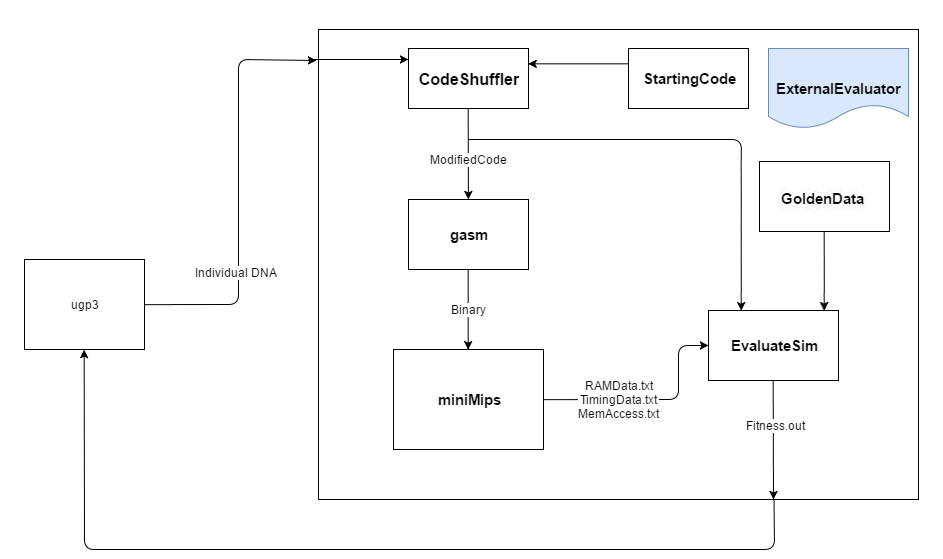
\includegraphics[scale=0.5]{Immagini/01}
\caption{uGP execution flow}
\end{figure}


\newpage


\section{Study cases}

\subsection{Unrolled Fibonacci}

\begin{lstlisting}
ADDI $31, $0, 0
LW $1, 1024($31)	# $1 <- nth

LUI $31, 1
SRL $31, $31, 14	# = 4
LW $2, 1024($31)	# $2 <- nth+1 (it's the index in the Fibonacci's serie)

ADD $1, $2, $1		# 2
SLL $31, $31, 1		# index <- 4*2
SW $1, 1024($31)

ADD $2, $2, $1		# 3
ADDIU $31, $31, 4	# index <- 12
SW $2, 1024($31)	# 

ADD $1, $2, $1		# 5
ADDI $31, $31, 4	# index <-16
SW $1, 1024($31)

ADD $2, $2, $1		# 8
ADDIU $31, $31, 4	# index <- 20
SW $2, 1024($31)	# 

ADD $1, $2, $1		# 13
ADDI $31, $31, 4	# index <- 24
SW $1, 1024($31)

ADD $2, $2, $1		# 21
ADDIU $31, $31, 4	# index <- 28
SW $2, 1024($31)	# 

ADD $1, $2, $1		# 44
ADDI $31, $31, 4	# index <- 32
SW $1, 1024($31)

ADD $2, $2, $1		# 65
ADDIU $31, $31, 4	# index <- 36
SW $2, 1024($31)	# 

end: j end
\end{lstlisting}

This program takes as inputs 2 numbers (i-th and i-th+1) owning to Fibonacci's 
series and generates the next 8 values. They have to store in the first and 
second ram location, respectively.
If the RAM starts at 1024, in terms of global addressing, we'll have
\begin{align*}
&1024(\$0) <= ith\\
&1028(\$0) <= ith+1
\end{align*}


The outputs are stored in RAM, as well. To see them you should read the content 
of the first tem RAM locations.
\begin{align*}
&1024(\$0) <= ith\\
&1028(\$0) <= ith+1\\
&1032(\$0) <= ith+2\\
&1036(\$0) <= ith+3\\
...
\end{align*}

\begin{figure}[H]
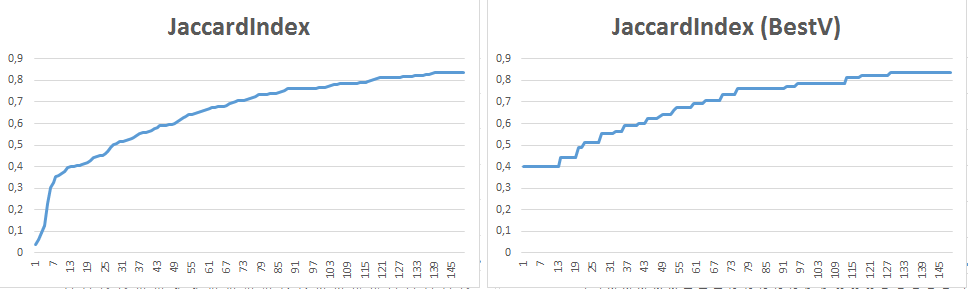
\includegraphics[scale=0.5]{Immagini/08}
\caption{Jaccard Index}
\end{figure}

\begin{figure}[H]
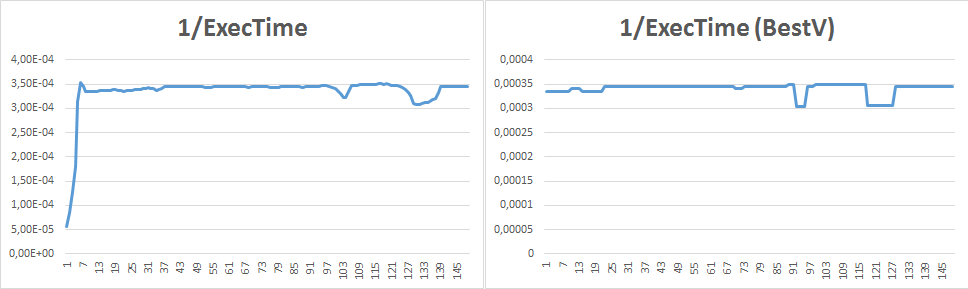
\includegraphics[scale=0.5]{Immagini/09}
\caption{Execution Time}
\end{figure}

\begin{figure}[H]
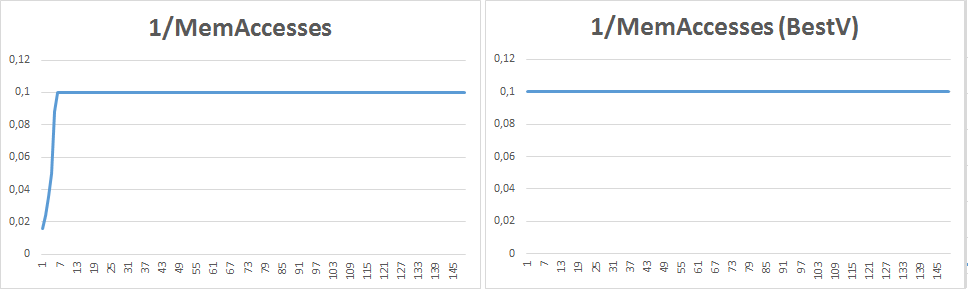
\includegraphics[scale=0.5]{Immagini/10}
\caption{Memory Accesses}
\end{figure}

In the initial code, there were 28 tuples.
In the final code, only 1 of those tuples are left.
96.42857\% of possible trojans have been mitigated. In fact, as said before, we don't know the actual sequence of instruction that actives the trojan. Assuming that the initial code contains one raising tuple, at the end of the process we have obtained a best (final) code where the probability of activating the malicious behaviour is dropped to around 95\%. We say it because we assumed that one of the 28 initial tuples was the offending one.

\newpage
\subsection{Average of 10 numbers}

\begin{lstlisting}
		addi $1, $0, 10		# initialize loop counter to 0
		addi $5, $0, 0		# initialize accumulator to 0	
label:		addi $1, $1, -1
		lw $3, 1024($2)		# load from memory
		add $5, $3, $5		# accumulate
		addi $2, $2, 4	
		bne $1, $0, label	# loop
		sll $10, $5, 7		# x * 128
		add $6, $10, $0		# 128 x
		sll $11, $5, 6		# x * 64
		add $6, $11, $6		# 192 x
		sll $12, $5, 3		# x * 8
		add $6, $12, $6		# 200 x
		sll $13, $5, 2		# x * 4
		add $6, $13, $6		# 204 x
		add $6, $5, $6		# 205 x
		srl $5, $6, 11		# 205x/2048 = x/10 
		sw $5, 1024($0)		
		sll $0, $0, 0		
end: 		j end
			
			

\end{lstlisting}

In the initial code, there were 20 tuples.
In the final code, only 0 of those tuples are left.
100\% of possible trojans have been mitigated. In fact, as said before, we don't know the actual sequence of instruction that actives the trojan. Assuming that the initial code contains one raising tuple, at the end of the process we have obtained a best (final) code that doesn't enable the malicious behaviour. We say it because we assumed that one of the 20 initial tuples was the offending one.

\newpage

\begin{figure}[H]
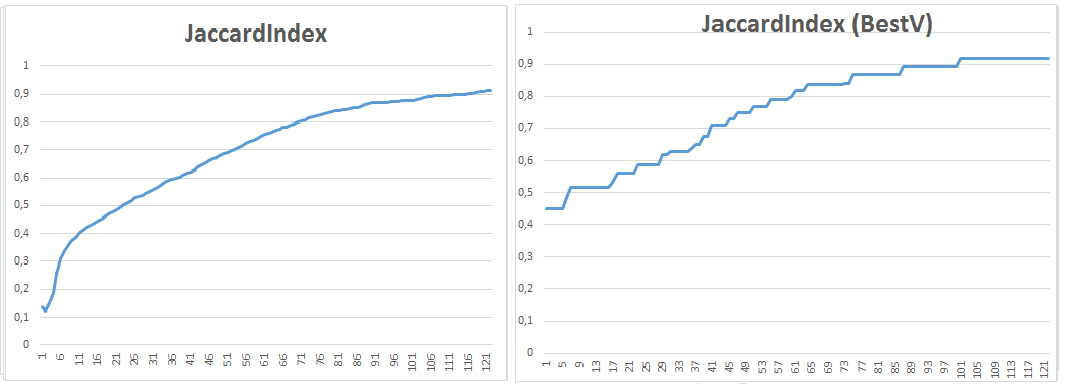
\includegraphics[scale=0.5]{Immagini/02}
\caption{Jaccard Index}
\end{figure}

\begin{figure}[H]
\raggedright
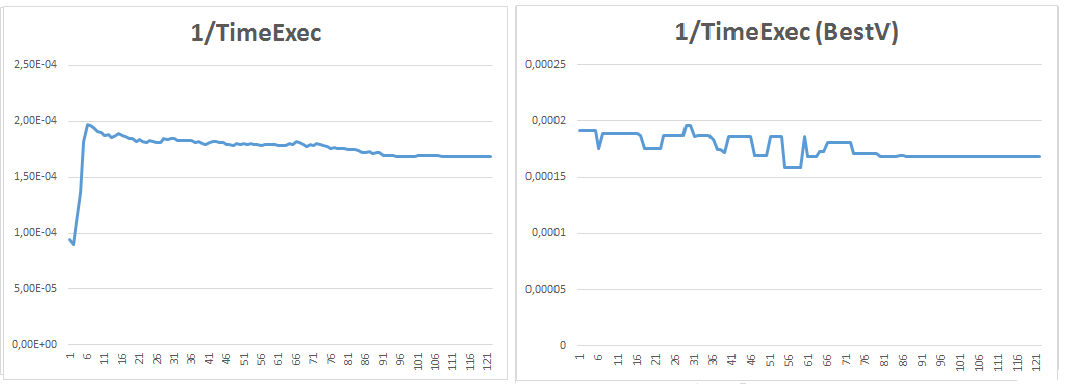
\includegraphics[scale=0.5]{Immagini/03}
\caption{Execution Time}
\end{figure}

\begin{figure}[H]
\raggedright
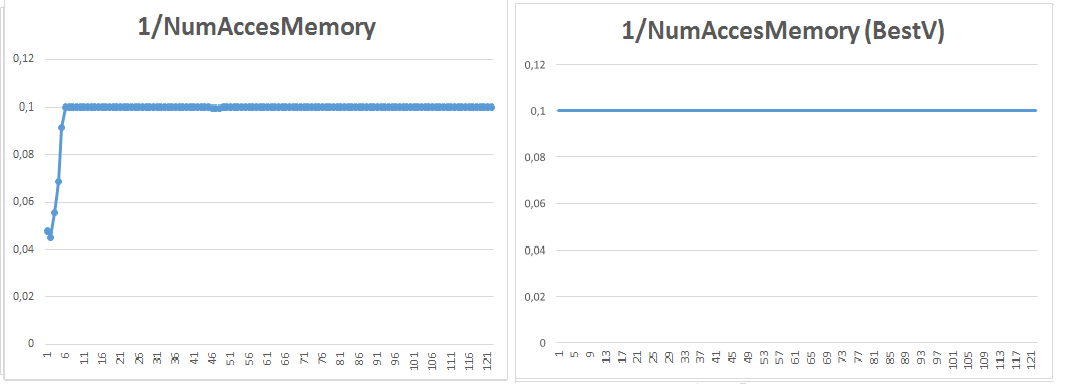
\includegraphics[scale=0.5]{Immagini/04}
\caption{Memory Accesses}
\end{figure}

\newpage

\subsection{Factorials}

\begin{lstlisting}
		addi $1, $0, 10		#counter elements
		addi $2, $0, 0		#pointer elements
	
loopelem:   	addi $1, $1, -1		#decrease counter fact
            	lw $3, 1024($2)		#load next value at.. 
             				#the address 1024 + $2(pointer)
            	addi  $4, $0, 2		#initialize factorial counter for...
            				# multiplications (starting from 2)
            	addi $5, $0, 1		#acc of fact(accf)
            	addi $3,$3,-1		#decrement the counter by one(starting...
            				#from 2 we have to compute A-1 multiplications 
            	add $8,$0,$0		#initialize the multiplication counter... 
            				#(multiplication implemented as a loop of additions

loopfact:   	addi $3,$3,-1		#decrement the factorial counter 
            	add  $6, $0, $5		#accumulator of factorial -> operand(that needs...
            				#to be summed continuosly to implement mult)
            	add  $7, $0, $4		#pointerf -> counterm
            	add  $8, $0, $0		#set the multiplication accumulator to 0
            	addi $4, $4, 1		#increment by one the factorial counter 

loopmul:    	addi $7, $7, -1		#decrease counter mul
            	add  $8, $8, $6		#accm=accm+operand
	    	bne $7, $0, loopmul	#if not finish, keep adding
	    	add $5 , $0, $8	#update the accf with the result of mult
	    	bne $3, $0, loopfact	#if not finish, keep multiplying
            	sw $5, 1024($2)		#store fact value to the same cell of memory
            	addi $2, $2, 4		#increase pointer fact
            	bne $1, $0, loopelem	#if not finish, keep taking elements from memory
			
end: 		j end			#conventional return instructional
			
			

			

\end{lstlisting}

In the initial code, there were 39 tuples.
In the final code, only 10 of those tuples are left.
74.35897\% of possible trojans have been mitigated. In according to written in the previous subsection, in this study case we have reduced the possibility of trojan enabling of around 74\%, but the threat is not vanquished at all. 

\newpage

\begin{figure}[H]
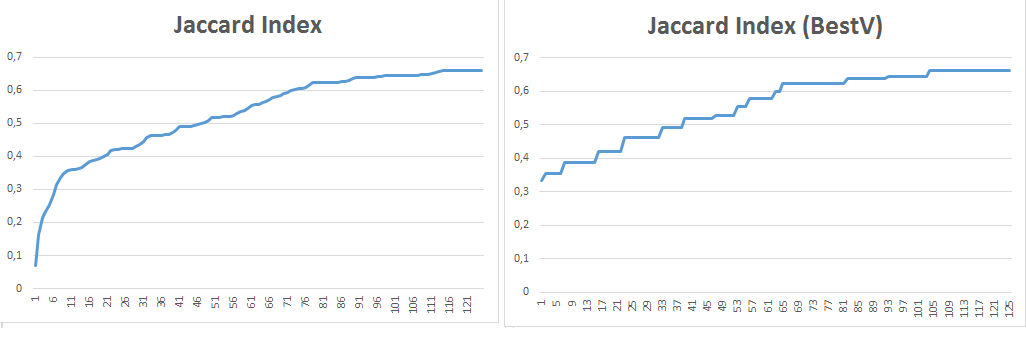
\includegraphics[scale=0.6]{Immagini/05}
\caption{Jaccard Index}
\end{figure}

\begin{figure}[H]
\raggedright
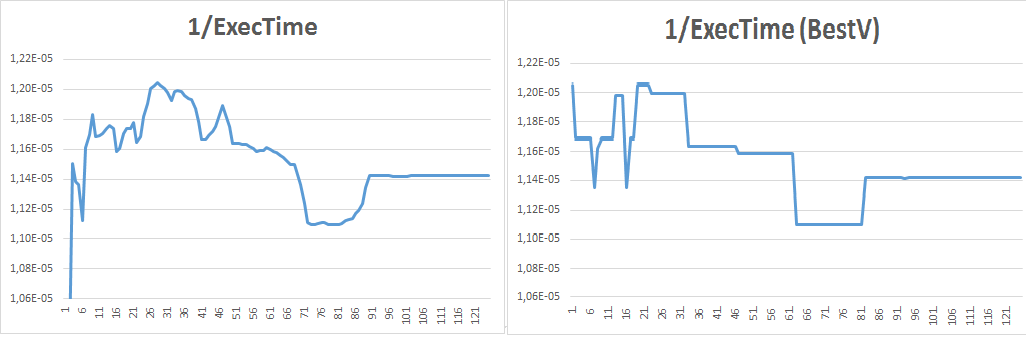
\includegraphics[scale=0.6]{Immagini/06}
\caption{Execution Time}
\end{figure}

\begin{figure}[H]
\raggedright
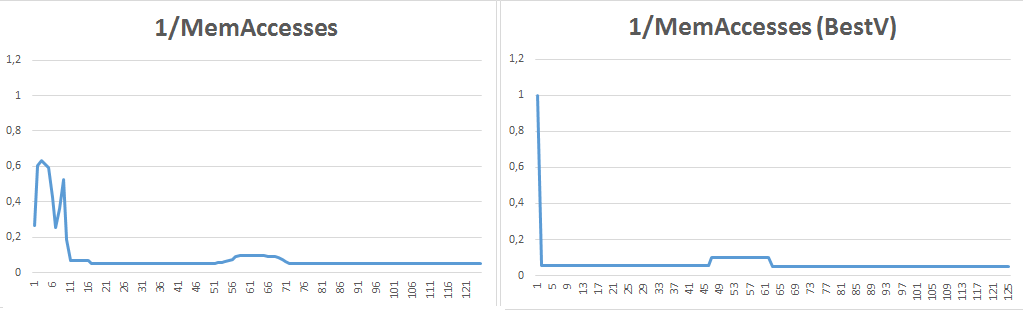
\includegraphics[scale=0.6]{Immagini/07}
\caption{Memory Accesses}
\end{figure}

\newpage

\subsection{Matrix product}

\begin{lstlisting}
XOR $31, $31,$31	# i
XOR $30, $30, $30	# j
XOR $29, $29, $29	# k
ADDI $28, $0, 2		# dim matrixes 
XOR $10, $10, $10	# counter
label: 
	   XOR $30, $30, $30
	   
	   label2:
			  XOR $29, $29, $29
			  label3:
					 
					 LW $3, 1056($0)
					 SLL $31, $31, 3
					 SLL $29, $29, 2
					 ADD $27, $31, $29
					 LW $1, 1024($27)	#mat1[i][k] 
					 SRL $31, $31, 3
					 SRL $29, $29, 2
					 SLL $29, $29, 3
					 SLL $30, $30, 2
					 ADD $26, $30, $29
					 LW $2, 1040($26)	#mat2[k][j] 
					 SRL $29, $29, 3
					 SRL $30, $30, 2
					 MULT $1, $2
					 			# MFHI $2
					 MFLO $4	        # STRONG ipothesis: 
					 #multiplication generates a number max 32-bit long
					 
					 ADD $3, $3, $4		
					 SW $3, 1056($0)
					 ADDI $29, $29, 1	
                                         SLL $0, $0, 0
					 bne $29, $28, label3   
                                         SLL $0, $0, 0
			  LW $3, 1056($0)
			  SW $3, 1060($10) 
 			  SW $0, 1056($0)
			  ADDI $10, $10, 4
			  ADDI $30, $30, 1	
			  SLL $0, $0, 0
			  bne $30, $28, label2
                          SLL $0, $0, 0
	   ADDI $31, $31, 1
	   SLL $0, $0, 0
	   bne $31, $28, label
           SLL $0, $0, 0	
XOR $10, $10, $10
ADDI $2, $0, 16
label4:	LW $1, 1060($10)	#this cycle is very useful only for debug purposes
        SW $1, 1024($10)
	ADDI $10, $10, 4
        SLL $0, $0, 0
	BNE $10, $2, label4

SLL $0, $0, 0		
end: j end
\end{lstlisting}

This program performs the matrix product between two matrices 2$\times$2. Let's 
imagine to have the following situation:

\begin{equation*}
\begin{bmatrix}
a_1 & a_2 \\ 
a_3 & a_4
\end{bmatrix}
\times
\begin{bmatrix}
b_1 & b_2 \\ 
b_3 & b_4
\end{bmatrix}
=
\begin{bmatrix}
c_1 & c_2 \\ 
c_3 & c_4
\end{bmatrix}
\end{equation*}

To use that, it is necessary to provide inputs $a_i$ and $b_i$, in according to the 
following implementative choice:
\begin{align*}
1024(\$0) <= a1 & & 1040(\$0) <= b1\\
1028(\$0) <= a2 & & 1044(\$0) <= b2\\
1032(\$0) <= a3 & & 1048(\$0) <= b3\\
1036(\$0) <= a4 & & 1052(\$0) <= b4\\
\end{align*}


At the end, $A$ matrix locations are replaced by the elements of the result one.

The execution time is estimated between 25000 ns and 26000 ns. 
This program uses  RAM addresses in range [1024, 1072].
\newline

In the initial code, there were 67 tuples.
In the final code, only 15 of those tuples are left.
77.61194\% of possible trojans have been mitigated.

\newpage

\begin{figure}[H]
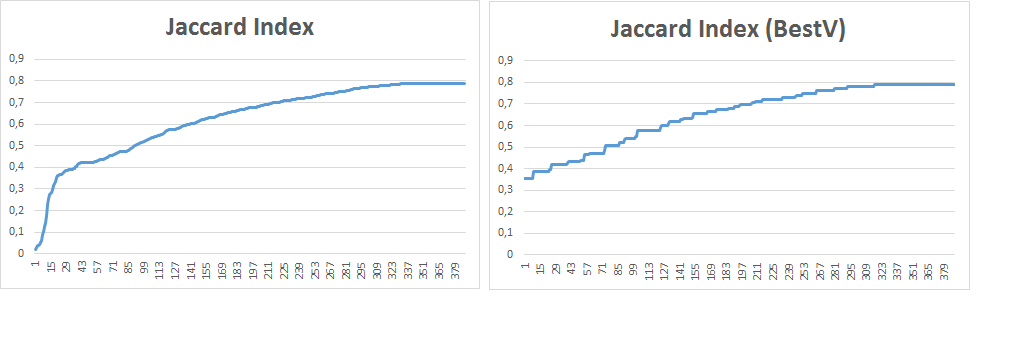
\includegraphics[scale=0.6]{Immagini/11}
\caption{Jaccard Index}
\end{figure}

\begin{figure}[H]
\raggedright
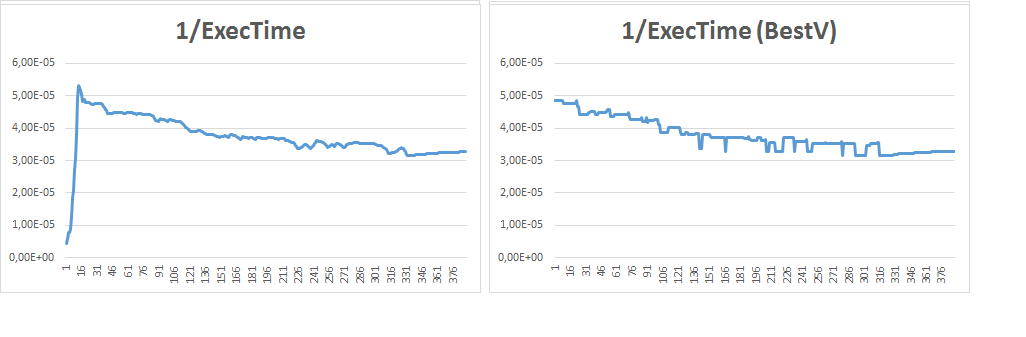
\includegraphics[scale=0.6]{Immagini/12}
\caption{Execution Time}
\end{figure}

\begin{figure}[H]
\raggedright
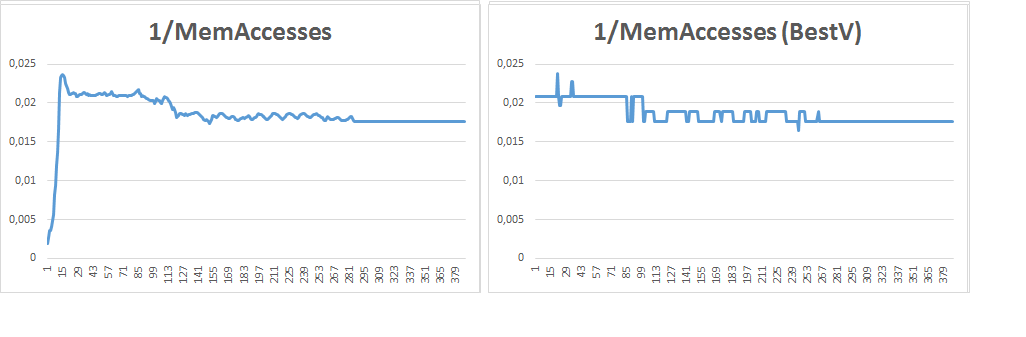
\includegraphics[scale=0.6]{Immagini/13}
\caption{Memory Accesses}
\end{figure}

In the initial code, there were 67 tuples.
In the final code, only 15 of those tuples are left.
77.61194\% of possible trojans have been mitigated.


\newpage
\appendix
\newpage
$\\$
\section{Instruction substitution table}


\begin{table}[H]
\centering
\begin{tabular}{|p{0.2\textwidth}|p{0.2\textwidth}|p{0.2\textwidth}|p{0.2\textwidth}|}
\hline
\textbf{Instruction format}&\textbf{Substitution 1 code}&\textbf{Substitution 2} & \textbf{Substitution 3}\\ \hline
ADD Rd, Rs, Rt& ADDU Rd, Rs, Rt & X & X \\  \hline
ADDI Rt, Rs, N& ADDIU Rt, Rs, N & X & X  \\  \hline
ADDIU  Rt, Rs, N& ADDI Rt, Rs, N & X & X  \\  \hline
ADDU Rd, Rs, Rt& ADD Rd, Rs, Rt &  X & X  \\  \hline
AND Rd, Rs, Rt& ANDI Rs, Rs, -1 \newline
                ANDI Rt, Rt, -1 \newline
                AND Rd, Rs, Rt&	
                XORI Rs, Rs, -1 \newline
                XORI Rt, Rt, -1	\newline
                OR Rd, Rs, Rt	\newline
                XORI Rd, Rd, -1	\newline
                XORI Rs, Rs, -1	\newline
                XORI Rt, Rt, -1 & X  \\  \hline
ANDI Rt, Rs, N& XORI Rs, Rs, -1 \newline
                ADD Rt, $0, Rs \newline
                ADDI Rs, $0, N \newline
                XORI Rs, Rs, -1 \newline
                NOR Rt, Rt, Rs &	
                ADDI Rt, \$0, N \newline
                XORI Rt, Rt, -1 \newline
                XORI Rs, Rs, -1 \newline
                NOR Rt, Rt, Rs \newline
                XORI Rs, Rs, -1& X  \\  \hline
BEQ Rs, Rt, offset& XOR Rs, Rs, Rt\newline
                    BEQ Rs, \$0, offset &
                    ADDI Rs, Rs, 1 \newline
                    ADDI Rt, Rt, 1 \newline
                    BEQ Rs, Rt, offset&
                    ANDI Rs, Rs, -1 \newline
                    BEQ Rs, Rt, offset
                      \\  \hline
BGEZ Rs, offset& BEQ Rs, \$0, offset\newline
                 BGTZ Rs, offset &
                 BEQ Rs, \$0, offset\newline
                 BGEZ Rs, offset & X  \\  \hline
BGEZAL Rs, offset& AND Rs, Rs, -1 \newline
                   BGEZAL Rs, offset &
                   OR Rs, Rs, 0 \newline
                   BGEZAL Rs, offset& X \\  \hline
BGTZ Rs, offset&  AND Rs, Rs, -1 \newline
                   BGTZ Rs, offset &
                   OR Rs, Rs, 0 \newline
                   BGTZ Rs, offset& X \\  \hline
BLEZ Rs, offset& BEQ Rs, \$0, offset\newline
                 BLTZ Rs, offset& 
                 AND Rs, Rs, -1\newline
                 BLEZ Rs, offset& 
                 OR Rs, Rs, 0\newline
                 BLEZ Rs, offset \\  \hline
BLTZ Rs, offset&   AND Rs, Rs, -1 \newline
                   BLTZ Rs, offset &
                   OR Rs, Rs, 0 \newline
                   BLTZ Rs, offset& X \\  \hline
BLTZAL Rs, offset & AND Rs, Rs, -1 \newline
                   BLTZAL Rs, offset &
                   OR Rs, Rs, 0 \newline
                   BLTZAL Rs, offset& X \\  \hline
BNE Rs, Rt, offset& XOR Rs, Rs, Rt \newline
                    BNE Rs, \$0, offset& X & X  \\  \hline
BREAK&X &	X & X \\  \hline
COP0 cop\_func&X &	X & X \\  \hline
J target &X &		X & X \\  \hline
JAL target &X &	X & X  \\  \hline
JALR Rd, Rs&X &	X & X  \\  \hline
JR Rs& AND Rs, Rs, Rs \newline
       JR Rs&		X & X  \\  \hline
LUI Rt, N&XOR Rs, Rs, Rs\newline
          ADDI Rs, Rs, N
          SLL Rs, Rs, 16 &	X & X \\  \hline
LW Rt, offset& XOR Rt, Rt, Rt\newline
               AND Rt, Rt, Rt\newline
               LW Rt, offset& 	X & X \\  \hline
LWC0 Cs, offset&X &	X & X  \\  \hline
MFC0 Rt, Cs&X &	X & X  \\  \hline
MFHI Rd& XOR Rd, Rd, Rd \newline
         MFHI Rd &	X & X  \\  \hline
MFLO Rd& XOR Rd, Rd, Rd \newline
         MFLO Rd &	X & X  \\  \hline
\end{tabular}
\caption{Instruction possible substitutions - I}
\end{table}
\begin{table}[H]
\centering
\begin{tabular}{|p{0.2\textwidth}|p{0.2\textwidth}|p{0.2\textwidth}|p{0.2\textwidth}|}
\hline
\textbf{Instruction format}&\textbf{Substitution 1 code}&\textbf{Substitution 2} & \textbf{Substitution 3}\\ \hline
MTC0 Rt, Cs&X &	X & X  \\  \hline
MTHI Rs&X &	X & X  \\  \hline
MTLO Rs&X &	X & X  \\  \hline
MULT Rs, Rt&MULTU Rs, Rt &	X & X  \\  \hline
MULTU Rs, Rt&MULT Rs, Rt &	X & X  \\  \hline
NOR Rd, Rs, Rt&OR Rd, Rs, Rt \newline
               XORI Rd, Rd, -1
 &	X & X \\  \hline
OR Rd, Rs, Rt&NOR Rd, Rs, Rt \newline
              XORI Rd, Rs, -1 &		X & X  \\  \hline
ORI Rt, Rs, N&ADDI Rt, \$0, N \newline
              NOR Rt, Rt, Rs &	X & X  \\  \hline
SLL Rd, Rt, N&ADDI Rd, \$0, N \newline
              SLLV Rd, Rd, Rt &	X & X  \\  \hline
SLLV Rd, Rt, Rs&ADDI Rd, \$0, Rs \newline
                SLL Rs, Rs, 1 \newline
                SLLV Rd, Rt, Rs&	X & X  \\  \hline
SLT Rd, Rs, Rt& SUB Rd, Rs, Rt\newline
                SRL Rd, Rd, 31 &	X & X \\  \hline
SLTI Rt, Rs, N&ADDI Rt, Rs, -N\newline
               SRL Rt, Rt, 31&	X & X  \\  \hline
SLTIU Rt, Rs, N& ADDIU Rt, \$0, N\newline
                 SLTU Rt, Rs, Rt&	X & X  \\  \hline
SLTU Rd, Rs, Rt&X &	X & X  \\  \hline
SRA Rd, Rt, N&ADDI Rd, \$0, N\newline
              SRAV Rd, Rt, Rd &	X & X \\  \hline
SRAV Rd, Rt, Rs&SRA Rt, Rt, 1\newline
                ADDI Rs, Rs, -1\newline
                SRAV Rd, Rt, Rs&	X & X \\  \hline
SRL Rd, Rt, N&ADDI Rd, \$0, N\newline
              SRLV Rd, Rt, Rd &	X & X  \\  \hline
SRLV Rd Rt, Rs& X&	X & X  \\  \hline
SUB Rd, Rs, Rt& XORI Rt, Rt, -1\newline
                ADD Rd, Rs, Rt \newline
                ADDI Rd, Rd, 1 \newline
                XORI Rt, Rt, -1&	X & X \\  \hline
SUBU Rd, Rs, Rt&SUB Rd, Rs, Rt&	X & X  \\  \hline
SW Rt, offset&XOR Rd, Rd, \$6 \newline
              XOR \$6, \$6, Rt \newline
              XOR Rt, Rt, \$6 \newline
              SW \$6, offset \newline
              XOR Rd, Rd, \$6 \newline
              XOR \$6, \$6, Rt \newline
              XOR Rt, Rt, \$6 
               & X & X  \\  \hline
SWC0 Cs, offset&X &	X & X  \\  \hline
SYSC &X &	X & X  \\  \hline
XOR Rd, Rs, Rt&XORI Rt, Rt, -1 \newline
               AND Rd, Rs, Rt \newline
               XORI Rt, Rt, -1 \newline
               XORI Rs, Rs, -1 \newline
               AND Rs, Rs, Rt \newline
               OR Rd, Rd, Rs \newline
               XORI Rs, Rs, -1 &	X & X  \\  \hline
XORI Rt, Rs, N&ADDI Rt, \$0, N \newline
               XOR Rt, Rs, Rt &	X &X \\  \hline
\end{tabular}
\caption{Instruction possible substitutions - II}
\end{table}
\end{document}
